\documentclass[12pt]{article}
\usepackage{amsmath}
\usepackage{amssymb}
\usepackage{amsthm}
\usepackage{amsfonts}
\usepackage{graphicx}
\usepackage{textcomp}
\usepackage{hyperref}
\usepackage{tikz}
\usepackage{enumitem}
\usepackage{mathtools}
\usepackage{enumitem}
\usepackage{wasysym}
\usepackage{ulem}
\usepackage{xspace}
\usepackage{csquotes}

\DeclareMathOperator{\dist}{dist}
\DeclareMathOperator{\Nul}{Nul}
\DeclareMathOperator{\Row}{Row}
\DeclareMathOperator{\proj}{proj}

\setlength{\arraycolsep}{12pt}

\newcommand{\defn}{\textbf{Def.}\xspace}
\newcommand{\thm}{\textbf{Thm.}\xspace}
\newcommand{\ex}{\textbf{ex.}\xspace}
\newcommand{\Ex}{\textbf{Ex.}\xspace}
\newcommand{\ie}{\textbf{i.e.}\xspace}
\newcommand{\lemma}{\textit{Lemma}\xspace}
\newcommand{\bproof}{\textit{Proof ($\impliedby$).}\xspace}
\newcommand{\fproof}{\textit{Proof ($\implies$).}\xspace}
\newcommand{\bigEps}{\mathcal{E}}
\newcommand{\soln}{\textit{Soln.}\xspace}

\renewcommand{\arraystretch}{1.25} % Adjust row spacing


\hypersetup{
    colorlinks=true,
    linkcolor=blue,
    filecolor=blue,      
    urlcolor=blue,
}

\newcommand{\ulhref}[2]{\href{#1}{\color{blue}\uline{#2}}}

\begin{document}

\title{MACM 316 Lecture 20}
\author{Alexander Ng}
\date{Wednesday, February 26, 2025}

\maketitle

\section{Approximation and Interpolation}

It is often useful or necessary to approximate a complicated or expensive function,
or a function only known at a discrete set of points, by a smpler function
which can be computed or evaluated more easily over a whole interval. When the
function in question is known accurately at a discrete set of points, we are
inclined to use an interpolation procedure- where the graph of the approximating 
function runs exactly through the points of the discrete set. 

If the dataset is expected to contain error, which is the case for measurements
or observations in experimental studies, a better strategy is to allow the
graph of the approximating function to stray from the data points.

% insert image here

A useful and well known class of functions for mapping the set of real numbers
into itself is the class of algebraic polynomials.

\[
  P_n(x) = a_nx^n + a_{n-1}x^{n-1} + \dots + a_1x + a_0
.\]

where $n$ is a non-negative integer and $a_i$ are real constants. Polynomials 
have the desirable property that they can approximate \uline{any} function
over a closed, bounded interval.

This desired property is precisely captured by the \textbf{Weierstrass 
Approximation Theorem}

\pagebreak

\subsection{The Weierstrass Approximation Theorem}

Suppose $f \in C[a,b]$. 

$\forall \bigEps > 0 \exists P \in \{ \mathbb{P}_n , C[a,b] \}$ such that

\[
  |f(x)-P(x)| < \epsilon \forall x \in [a,b]
.\]

\begin{figure}[h]
    \centering
    \resizebox{0.8\textwidth}{!}{%
        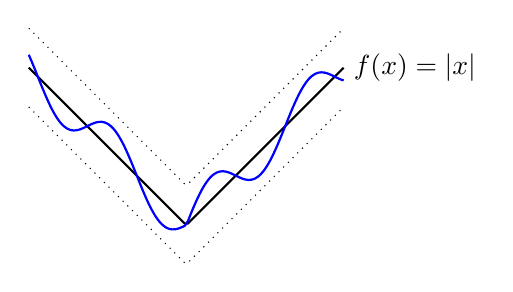
\begin{tikzpicture}
            % Define the function
            \draw[thick] plot[samples=100,domain=-2:2] (\x,{abs(\x)}) node[right] {$f(x) = |x|$};

            % Epsilon bounds
            \draw[dotted] plot[samples=100,domain=-2:2] (\x,{abs(\x) + 0.5});
            \draw[dotted] plot[samples=100,domain=-2:2] (\x,{abs(\x) - 0.5});

            % Labeling epsilon
            % \draw[->] (1,1.5) -- (1.1,1.2) node[midway,right] {$\varepsilon$};
            % \draw[->] (-1,1.5) -- (-1.1,1.2) node[midway,left] {$\varepsilon$};

            % Approximation function (squiggly)
            \draw[thick,blue] plot[smooth, samples=100, domain=-2:2] (\x, {0.3*sin(5*\x r) + abs(\x)});

        \end{tikzpicture}%
    }
    \caption{Polynomial approximation to $f(x) = |x|$.}
\end{figure}

This is a very strong theorem, as it only requires $f(x)$ to be continuous on 
the interval, and not necessarily differentiable.

Unfortunately, the Weierstrass Approximation Theorem does not tell us how to 
select such a polynomial. Many would immediately jump to using Taylor series
polynomials for polynomial interpolation, however, Taylor series' concentrate
their accuracy at the point $a$ rather than over the entire interval, and are
typically poorly suited for interpolation.

\subsubsection{Taylor Series Polynomials}

\[
P_n(x) = f(a) + f'(a)(x-a) + \frac{f''(a)}{2!}(x-a)^2 + \dots + \frac{f^{(n)}(a)}{n!}(x-a)^n
.\]

A particularly clear demonstration of this drawback is seen for

\[
f(x) = \frac{1}{x} \qquad \text{expanded about } x_0 = 1
.\]

Then,

\begin{align*}
  P_n(x) &= \sum_{k=0}^n \frac{f^{(k)}(1)}{k!}(x-1)^k\\
         &= \sum_{k=0}^n (-1)^k(x-1)^k \\
\end{align*}

To approximate $f(3)=\frac{1}{3}$ by $P_n(3)$ for increasing values of $n$, we
see a dramatic and catastrophic failure: 

\begin{table}[h]
    \centering
    \renewcommand{\arraystretch}{1.4}
    \begin{tabular}{|c|c|c|c|c|c|c|c|c|}
        \hline
        \( n \) & 0 & 1 & 2 & 3 & 4 & 5 & 6 & 7 \\ 
        \hline
        \( P_n(3) \) & 1 & -1 & 3 & -5 & 11 & -21 & 43 & -85 \\ 
        \hline
    \end{tabular}
    \caption{Values of \( P_n(3) \) for increasing \( n \).}
\end{table}

We will insetad focus on methods which use information throughout the entire 
interval to approximate $f$.

\section{Polynomial Interpolation}

We now assume that the given dataset is exact and represents values of some
unknown function. We want to find the polynomial $P_n(x)$ of the smallest 
possible degree $n$ such that

\[
P_n(x_k) = f_k \qquad k = 1,2, \dots, N
.\]

for $N+1$ distinct interpolation points $x_0,\dots,x_N$ and $N+1$ values 
$\underbrace{f_0,\dots,f_N}_{\text{data points}}$.

To solve this problem, we will first investigate the simpler problem where all
the data equals zero, except at one point.

We are looking for a polynomial $L_m(x)$ of degree $\leq N$ such that

\[
  L_m(x_k) = \delta_{mk} \qquad = \begin{cases}
    1 & k = m \\
    0 & k \neq m
    \end{cases}
.\]


\begin{center}

\begin{tikzpicture}[overlay, remember picture]
    \draw[thick,->] (0,0) node[below]{\textbf{Kronecker Delta}} to (-1.1,0.8);
\end{tikzpicture}
\end{center}

This is easy to find. Since the polynomial must vanish at the points 
$x_k, k\neq m$, it must contain the factors

\[
  (x-x_k) \qquad \text{for } k \neq m
.\]

\[
\therefore L_m(x) = c \cdot \prod_{k=0; k\neq m}^N(x-x_k)
.\]

The constant is determined by the condition $L_m(x_m) = 1$.

\[
\implies L_m(x) = \prod_{k=0; k\neq m}^{N}  \frac{x-x_k}{x_m-x_k}
.\]

Typically, 
\begin{center}
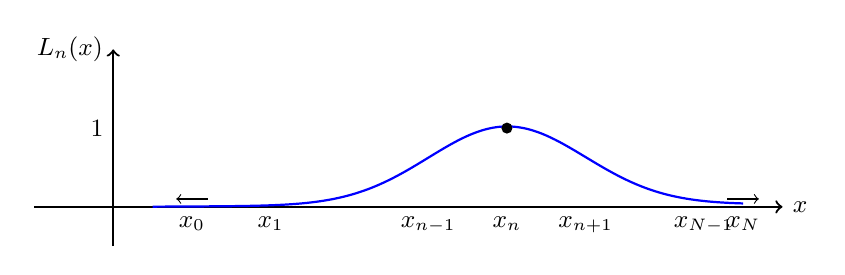
\begin{tikzpicture}
    % Axes
    \draw[thick,->] (-1,0) -- (8.5,0) node[right] {\small $x$}; % x-axis
    \draw[thick,->] (0,-0.5) -- (0,2) node[left] {\small $L_n(x)$}; % y-axis

    % Labels on axes
    \node[left] at (0,1) {\small 1}; % Label at y = 1

    % Points on x-axis
    \foreach \x/\label in {1/$x_0$, 2/$x_1$, 4/$x_{n-1}$, 5/$x_n$, 6/$x_{n+1}$, 7.5/$x_{N-1}$, 8/$x_N$}
        \node[below] at (\x,0) {\small \label};

    % Sinusoidal-like Lagrange basis function
    \draw[thick,blue,domain=0.5:8,samples=100,smooth] 
        plot (\x, {exp(-0.5*(\x-5)^2) * cos(2*pi*(\x-5)/3) + 0.05*sin(5*\x)});

    % Highlight peak at x_n
    \fill (5,1) circle (2pt);
    
    % Small arrows at edges
    \draw[->] (7.8,0.1) -- (8.2,0.1);
    \draw[->] (1.2,0.1) -- (0.8,0.1);
    
\end{tikzpicture}
\end{center}

These polynomials are the building blocks for deriving a polynomial
interpolating a general function. It is easy to see that

\[
  P(x) = \sum_{m=0}^N f_m < L_m(x)
.\]

is a polynomial of degree $\leq N$ satisfying the interpolation conditions.

This polynomial is called the $n^{th}$ \textbf{Lagrange Interpolating Polynomial} 

Recall that we wanted to find the polynomial $P_n(x)$ of smallest degree such
that 

\[
  P_n(x_k) = f_k \qquad k = 0,\dots,N
.\]

\subsection{Uniqueness}

Is this polynomial unique?

\textbf{Yes.} 

\proof Assume there are two different polynomials $p$ and $q$ of degree $\leq N$
which both satisfy the interpolation conditions. Their difference, $d=p-q$, is
also a polynomial of degree $\leq N$ and vanishes at the $N+1$ distinct points 
$x_0,\dots,x_N$.

However, a nonzero polynomial of degree $\leq N$ has at most $N$ zeros, this

\[
d = p-q = 0 \implies \begin{cases}
  p=q\\
  \text{ uniqueness}
\end{cases}
\]

$\therefore$ the $n^{th}$ Lagrange Interpolating Polynomial is the unique
interpolating polynomial satisfying the interpolation conditions.

\subsection{Example}

Fit a cubic through the first four points of the table 

\begin{table}[h]
    \centering
    \begin{tabular}{c|c|c}
        $i$ & $x^i$ & $f(x_i)$ \\
        \hline
        0 & 3.2 & 22.0 \\
        1 & 2.7 & 17.8 \\
        2 & 1.0 & 14.2 \\
        3 & 4.8 & 38.3 \\
        4 & 5.6 & 51.7 \\
    \end{tabular}
    % \caption{Tabular representation of given data}
    % \label{tab:data}
\end{table}

and use it to find the interpolated value for $x=3.0$.

\soln The $3^{rd}$ Lagrange Interpolating Polynomial is given by

\begin{align*}
    P(x) = &\ \frac{(x - x_1)(x - x_2)(x - x_3)}{(x_0 - x_1)(x_0 - x_2)(x_0 - x_3)} f_0 \\
    &+ \frac{(x - x_0)(x - x_2)(x - x_3)}{(x_1 - x_0)(x_1 - x_2)(x_1 - x_3)} f_1 \\
    &+ \frac{(x - x_0)(x - x_1)(x - x_3)}{(x_2 - x_0)(x_2 - x_1)(x_2 - x_3)} f_2 \\
    &+ \frac{(x - x_0)(x - x_1)(x - x_2)}{(x_3 - x_0)(x_3 - x_1)(x_3 - x_2)} f_3
\end{align*}

Substituting the values from the table and evaluating at $x=3.0$ gives 

\begin{align*}
    P(3.0) = &\ \frac{(3.0 - 2.7)(3.0 - 1.0)(3.0 - 4.8)}{(3.2 - 2.7)(3.2 - 1.0)(3.2 - 4.8)} (22.0) \\
    &+ \frac{(3.0 - 3.2)(3.0 - 1.0)(3.0 - 4.8)}{(2.7 - 3.2)(2.7 - 1.0)(2.7 - 4.8)} (17.8) \\
    &+ \frac{(3.0 - 3.2)(3.0 - 2.7)(3.0 - 4.8)}{(1.0 - 3.2)(1.0 - 2.7)(1.0 - 4.8)} (14.2) \\
    &+ \frac{(3.0 - 3.2)(3.0 - 2.7)(3.0 - 1.0)}{(4.8 - 3.2)(4.8 - 2.7)(4.8 - 1.0)} (38.3) \\
    &= 20.21
\end{align*}

Our next task is to develop estimates for the error. As it turns out, the form
of the error (but not necessarily the magnitude) resembles that of the $n^{th}$
Taylor Polynomial.

\subsection{Error Estimates}

*The lecture ended just before this section*

\thm (3.3 of Text)

Suppose $x_0, \dots, x_n$ are distinct numbers in the interval $[a,b]$ and
$f\in C^{n+1}[a,b]$. Then for each $x\in [a,b]$, a number $\xi(x)\in(a,b)$
exists with the property

\[
  f(x) = P(x) + \frac{f^{(n+1)}(\xi(x))}{(n+1)!} (x-x_0) (x-x_1) \dots (x-x_n)
.\]

\begin{center}

\begin{tikzpicture}[overlay, remember picture]
    \draw[thick,->] (-2,0) node[below]{\textbf{n-th Langrange Interpolating Polynomial}} to (-3.2,0.6);
\end{tikzpicture}
\end{center}

*do you guys like my diagrams with arrows?*

\end{document}
